\documentclass[11pt]{article}

\usepackage{float}
\usepackage{hyperref}
\usepackage{graphicx}
% formatting
\usepackage{fullpage}
\usepackage{verbatim}
\usepackage{moreverb}
\usepackage{minted}
\let\verbatiminput=\verbatimtabinput
\def\verbatimtabsize{4\relax}

\begin{document}
\title{EECS 151/251A FPGA Lab\\
Lab 1: Introduction to FPGA Development + Creating a Tone Generator}

\author{Prof. Borivoje Nikolic \\
TA: Vighnesh Iyer \\Department of Electrical Engineering and Computer Sciences\\
College of Engineering, University of California, Berkeley}
\date{}
\maketitle

\section{Before You Start This Lab}

Before you proceed with the contents of this lab, be sure that you have gone through and completed the steps involved in Lab 0. There is no checkoff for Lab 0, but there will be for this lab. Let the TA know if you are not signed up for this class on bCourses and Piazza or if you do not have a class account (eecs151-xxx), so we can get that sorted out. Also, please go through the Verilog Primer slides that are linked to on Piazza; you should feel somewhat comfortable with the basics of Verilog to complete this lab.\\

To fetch the skeleton files for this lab \verb|cd| to the git repository (\verb|labs_fa16|) that you had cloned in Lab 0 and execute the command \verb|git pull|.\\

You can find the documents/datasheets useful for this lab in the \verb|labs_fa16/docs| folder.

\section{Our Development Platform - Xilinx ML505}
For the labs in this class, we will be using the Xilinx XUPV5-LX110T development board which is built on the ML505 evaluation platform. Our development board is a printed circuit board that contains a Virtex-5 FPGA along with a host of peripheral ICs and connections. The development board makes it easy to program the FPGA and allows us to experiment with different peripherals. The following image identifies important parts of the board:

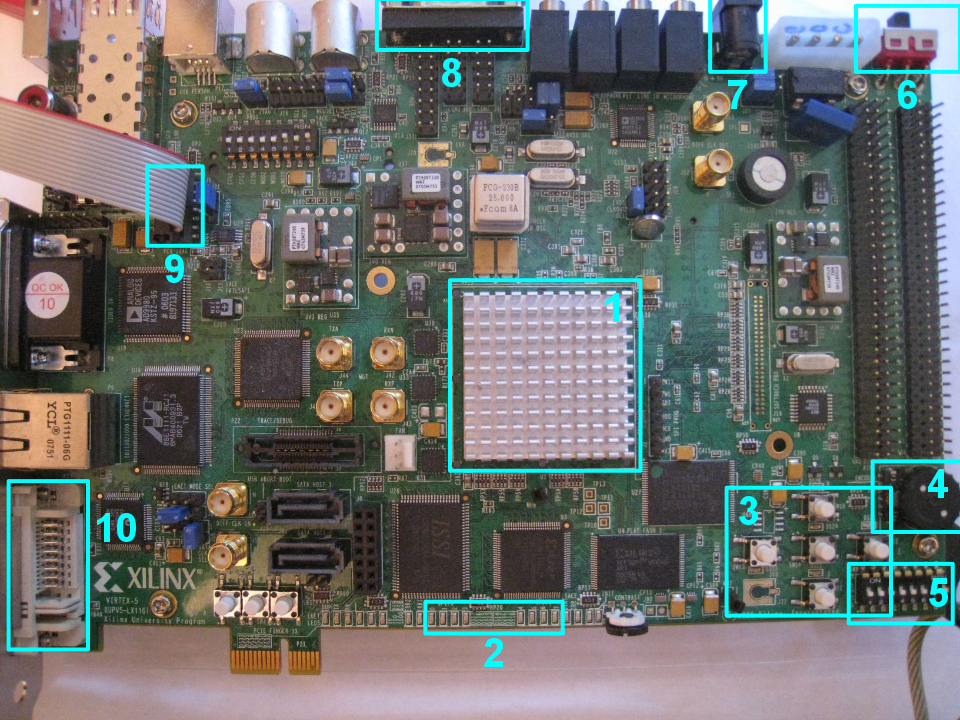
\includegraphics[width=\textwidth]{images/dev_board.png}
\begin{enumerate}
	\item Virtex-5 FPGA (covered by heat sink). It is connected to the peripheral ICs and I/O connectors via PCB traces.
	\item GPIO LEDs, numbered 0-7
	\item North, East, South, West, Center user push buttons, each with a corresponding LED
	\item Rotary encoder (a wheel we can rotate clockwise or counterclockwise and push horizontally)
	\item GPIO DIP (dual-inline package) switches, numbered 1-8 (but referred to 0-7 in code)
	\item Board power switch (toggle for a full board reset, after which you will have to reprogram the FPGA)
	\item Power connector; the power cable on many of these board is sensitive to movement and can come loose easily. Make sure you seat the power cable properly.
	\item Serial port
	\item JTAG header (used to program the FPGA, the Xilinx programmer is connected to this header)
	\item DVI-I connector (for video output)
\end{enumerate}

You will also notice a device sitting to the left of the development board that looks like this:\\

\begin{center}
	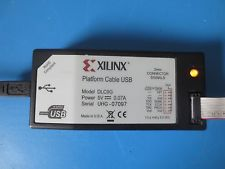
\includegraphics{images/xilinx_platform_cable.jpg}
\end{center}

This is a Xilinx FPGA programmer that connects to your workstation (desktop computer) over USB to receive a compiled bitstream file which it then sends to the development board and the FPGA over the JTAG interface. Before you run \verb|make impact| to send your design to the FPGA, make sure that the LED on the programmer is glowing green. If it is glowing yellow or not glowing at all, make sure that the wired connections are solid and that the development board is powered and on.

\section{The FPGA - Xilinx Virtex-5 LX110T}
To help you become familiar with the FPGA that you will be working with through the semester, please read Chapter 5: Configurable Logic Blocks (page 171) of the \href{http://inst.eecs.berkeley.edu/~cs150/fa11/resources/ug190.pdf}{Virtex-5 User Guide} and answer the following questions (you should be able to discuss your answers for checkoff):

\subsection{Checkoff Questions}
\begin{enumerate}
	\item How many SLICEs are in a single CLB?
	\item How many inputs do each of the LUTs on a Virtex-5 LX110T FPGA have?
	\item How many LUTs does the LX110T have?
	\item How do you implement logic functions of 7 inputs in a single SLICEL? How about 8? Draw a high-level circuit diagram to show how the implementation would look. Be specific about the elements (LUTs, muxes) that are used.
	\item What is the difference between a SLICEL and a SLICEM?
\end{enumerate}

\section{Overview of the FPGA Build Toolchain}
Before we begin the lab, we should familiarize ourselves with the CAD (computer aided design) tools that translate HDL into a working circuit on the FPGA. These tools will pass your design through several stages, each one bringing it closer to a concrete implementation.\\

Looking at the directory structure of the \verb|lab1| folder, you can see two main folders, \verb|src| and \verb|cfg|. You will also find a \verb|Makefile|. When executing parts of the toolchain, you will want to run \verb|make| in the \verb|lab1| folder. The \verb|Makefile| delegates to another \verb|Makefile| that resides in the \verb|cfg| folder. In the \verb|cfg| folder you will also find other files that are used by tools during the build process. We will discuss every step of the toolchain.\\

\subsection{Synthesis with XST}
The synthesis tool (in this case of this class, Xilinx Synthesis Tool(xst)) is the first program that processes your design. Among other tasks, it is responsible for the process of transforming the primitive gates and flip-flops that you wrote in Verilog into LUTs and other primitive FPGA elements.\\

For example, if you described a circuit composed of many gates, but ultimately of 6 inputs and 1 output, xst will map your circuit down to a single 6-LUT. Likewise, if you described a flip-flop it will be mapped to a specific type of flip-flop which actually exists on the FPGA.\\

The following figure shows the flow of files through XST. \\

\begin{center}
	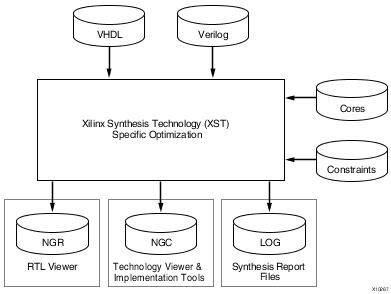
\includegraphics{images/xst_design_flow.png}
\end{center}

XST takes in Verilog and/or VHDL files to be parsed and synthesized.

XST also takes in 'Cores' which are pre-built and synthesized digital circuit blocks that provide some commonly needed functionality; they are usually provided by Xilinx to enable rapid FPGA development. They include things like pipelined dividers and multipliers, floating point units, and system buses.

XST also takes in 'Constraints' which are given in the form of a XCF file. In this lab, we don't use any constraints or cores that are passed into XST.

The outputs of XST include a LOG file, which is a text file that you can examine to make sure the synthesis succeeded, or if it failed or emitted warnings, you can see what those issues are.

Another output of XST is a NGR file which can be viewed with Xilinx ISE (as we will see soon); this file gives a high-level schematic view of how your Verilog modules are set to be implemented on the FPGA.

The final product of synthesis is a netlist file (NGC); it is a text file that contains a list of all the instances of primitive components in the translated circuit and a description of how they are connected.

\subsection{Translation and Mapping with NGDBuild and Map}
The tools that perform translation and mapping are NGDBuild and Map respectively. These tools take the output of the synthesis tool (a generic netlist) and translates each LUT and primitive FPGA element to an equivalent on the specific Xilinx vc5vlx110t FPGAs we have in the lab. 

The translation tool merges all the input netlists and design constraint information and outputs a Xilinx Native Generic Database (NGD) file. NGDBuild takes the UCF (User Constraints File) and the NGC (from XST) files as inputs.

The mapping tool maps the logic defined by an NGD file into FPGA elements such as CLBs (configurable logic blocks) and IOBs (input/output blocks). The Map tool takes in the NGD file produced by the translation tool and produces a Xilinx Native Circuit Description (NCD) file.

\subsubsection{User Constraints File (UCF)}
We will take a small detour here to cover what a UCF is and how to add top-level signal connections to it.

A user constraints file is passed to the translation tool (NGDBuild) and it contains information regarding the top-level pin assignments and timing constraints. When you opened \verb|ml505top.v| in Lab 0, you noticed that your top-level Verilog module received several input and output signals. These signals were \verb|input [7:0] GPIO_DIP| and \verb|output [7:0] GPIO_LED|. You added some Verilog gate primitives to drive the outputs with some logic operations done to the inputs. But how do the tools know where those signals come from? That's what the UCF is for.

Open the UCF \verb|lab0/ml505top.ucf| for Lab 0 and take a look. Here you can see where the \verb|GPIO_DIP| and \verb|GPIO_LED| nets come from. Here is the syntax used to declare a top-level signal that you can sense and/or drive from your top-level Verilog module.

\begin{minted}{verilog}
	NET (net name)<bit index> LOC="(FPGA pin number)"
	NET (net name)<bit index> IOSTANDARD="(voltage level)"
\end{minted}

The (net name) is the signal name that is presented to your top-level Verilog module. The bit index can be set optionally for a multi-bit signal for the same net name. The LOC defines what pin coming out of the FPGA contains that signal. All the pins coming out of the FPGA's BGA package are labeled, and this is how we can tap or drive signals from a particular pin. The second line defines an IOSTANDARD for a given net; this is just a statement of the voltage level for a given pin. Here is an example for a \verb|GPIO_LED|

\begin{minted}{verilog}
NET GPIO_LED<0> LOC="H18";
NET GPIO_LED<0> IOSTANDARD="LVCMOS25";
\end{minted}

These 2 lines give you access to a net called \verb|GPIO_LED| in your top-level Verilog module. This net is connected to the \verb|H18| pin coming out of the FPGA which is routed on the PCB to LED0 on the board via a trace.

Note that this declaration doesn't specify whether the net is an input or output; that is defined in your Verilog top-level module port declaration.

On the ML505 development board, we can utilize what is called a master UCF file to make adding signals to your design easy. This master UCF file is used in conjunction with the ML505 user guide and ML505 schematic to figure out what peripheral connections you want brought into your FPGA design. You can find these three files in the \verb|labs_fa16/docs| directory. We will discuss how to use these files in the design exercise in this lab.

\subsection{Place and Route with PAR}
Now we resume where we left off after the mapping tool. The map tool's NCD output file is fed into the Place and Route tool which is called PAR. PAR places and routes the design that was generated by Map, and it outputs another NCD file with placement and routing information. This process is often the most time consuming of any of the steps in the toolchain; the algorithms used for placement and routing are quite sophisticated and have long run times.

\subsection{Bitstream Generation with BitGen}
The fully placed and routed design from PAR as a NCD file is now ready to be translated into another file that the Xilinx FPGA programmer can understand. We use a tool called BitGen to perform the generation of the bitstream that is sent to the FPGA. This is the last step in the FPGA build process, and it produces a .bit file which can be uploaded to the FPGA via the programmer.

\subsection{Timing Analysis with TRCE}
The \verb|Makefile| we use in this class performs an additional step after running BitGen. To verify that our design met all timing requirements and to see a timing analysis, we use a tool called Trace (TRCE) which takes in output files generated by PAR and produces a timing report. It will let you know what is the maximum clock speed your design can operate at reliably.

\subsection{Report Generation with ISE}
A very important precaution to take after running each step of the toolchain is to verify that there are no errors or warnings that a given tool produced. We use a program called xreport which ships with Xilinx ISE to produce a report detailing the status of each build tool. To run this tool, execute \verb|make report| in the \verb|/lab1| directory. The tool will give you all the warnings and errors emitted by each tool in a GUI. It will also report the resource usage of your design.

\subsection{FPGA Programming with iMPACT}
Finally, to send the bitstream file you generated with BitGen to the FPGA, we use a tool called iMPACT. To execute this tool run \verb|make impact| in the \verb|/lab1| directory after the regular \verb|make| process has completed and succeeded without any errors. iMPACT will send your bitstream file to the FPGA programmer over USB, and the FPGA programmer will send the bitstream to the FPGA over JTAG. After this tool runs, your design will be configured and active on the FPGA.

\subsection{Toolchain Conclusion}
All of this information is dense and complex. Don't worry about understanding the internals of each tool and the exact file formats they work with. Just understand what each step of the toolchain does at a high level and you will be good for this class. We use all these tools regularly, but executing them is all handled by the staff provided \verb|Makefile|.


\section{A Structural and Behavioral Adder Design + Using fpga\_editor and the FPGA schematic}

\subsection{Build a Structural 4-bit Adder}
To help you with this task, please refer to the 'Code Generation with for-generate loops' slide in the Verilog Primer Slides (slide 35). You do not need to use for-generate loops to complete this task, but they will make it easier.\\

Navigate to the \verb|/lab1/src| directory. Begin by opening \verb|full_adder.v| and fill in the logic to produce the full adder outputs from the inputs. Then open \verb|structural_adder.v| and construct a ripple carry adder using the full adder cells you designed earlier. You can manually instantiate four instances of the full adder cell or you can use a for-generate statement. You can add as many internal wires to your module as you want.

Finally, inspect the \verb|ml505top.v| top-level module and see how your structural adder is instantiated and hooked up to the top-level signals.

Run \verb|make| in the \verb|/lab1| directory and let the build process complete. Then run \verb|make impact| to send your design to the FPGA. Test out your design and see that you get the correct results from your adder. You should try entering different binary numbers into your adder with the DIP switches and see that the correct sum is displayed on the first 5 LEDs. 

\subsection{Inspection of Structural Adder Using Schematic and fpga\_editor}
Now let's take a look at how the Verilog you wrote mapped to the primitive components on the FPGA. To do this, we will first look at a high-level schematic of your circuit using Xilinx ISE.\\

Execute the command \verb|make schematic| in the \verb|/lab1| directory. This will launch the ISE project navigator. Once inside ISE, go to \verb|File -> Open| and select \verb|ml505top.ngr|. You will recall that the NGR file is an output of XST (synthesis). Choose \verb|Start with a schematic of the top-level block| in the dialog that pops up.

This will given you a fairly straightforward hierarchical block-level view of your design. You will find your circuit by drilling down in the following modules: \verb|ml505top, st_add, full_adder|. Check to see that your structural adder module is hooked up properly and looks sane. It's ok if the wires aren't connected, just hover your mouse over the endpoints on the schematic and ensure that the connections are as you expect. Take note of the primitive blocks in your circuit.\\

Now let's take a look at how your circuit was placed and laid out on the FPGA with the \verb|fpga_editor|. Recall that the \verb|.ncd| file is the final result of the FPGA toolchain flow. There also exists a \verb|.pcf| file (Physical Constraints File) that contains the information originally present in the UCF, that is the locations of the I/O pins on the FPGA. By opening these files in the FPGA editor, you can visualize how your design will actually be mapped to the FPGA. Run these commands.

\begin{minted}{bash}
	cd lab1/build/ml505top
	DISPLAY=:0 fpga_editor ml505top.ncd ml505top.pcf
\end{minted}

\begin{center}
	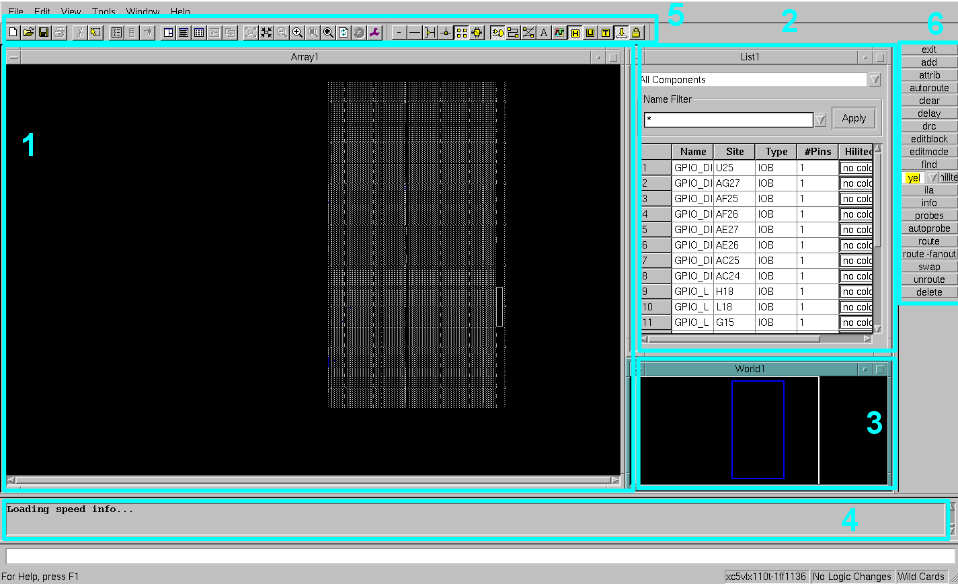
\includegraphics[width=\textwidth]{images/fpga_editor_1.png}
\end{center}

The image above shows the main view for the FPGA editor. It is split up into the following windows:

\begin{enumerate}
	\item \textbf{Array Window} - shows a schematic of the FPGA and highlights the parts of the FPGA that are currently utilized, as well as the connections between these components.
	\item \textbf{List Window} - lists the components and nets that are used in your design. Double-clicking items here will zoom in on them in the Array Window.
	\item \textbf{World Window} - this shows you where you are currently focused in the Array Window.
	\item \textbf{Console Output} - prints messages that often contain useful diagnostic information.
	\item \textbf{Toolbar} - contains useful buttons for manipulating the windows; mouse over the buttons to reveal what is does.
	\item \textbf{Button Bar} - contains other useful buttons for modifying the design.
\end{enumerate}

Now you can explore your design and look for the modules that you wrote. If you scroll down in the \verb|List Window| you will find that the type of some items is SLICEL.

Recall that SLICELs contain the look-up tables that actually implement the logic you want. Double clicking on the SLICEL named \verb|GPIO_LED_0BUF| will take you to the corresponding SLICEL in your Array Window. Double click on the red rectangle (the SLICEL) to bring up the following Block Window:

\begin{center}
	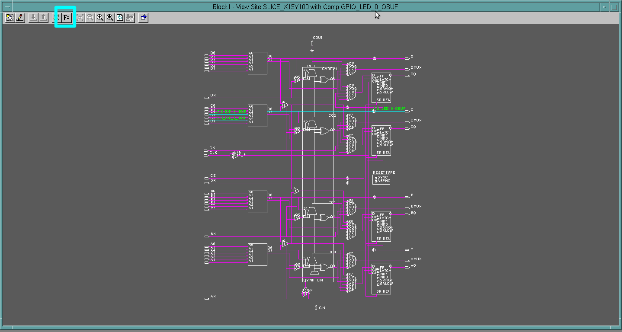
\includegraphics[width=\textwidth]{images/fpga_editor_2.png}
\end{center}

Click on the \verb|F=| button to reveal the function of the LUT. Go ahead and explore several SLICELs to see how they are connected to each other and the outputs of your circuit.\\

Finally you should run \verb|make report| to collect resource usage information for your structural design. Record the number of LUTs used.

\subsection{Build a Behavioral 4-bit Adder}

Check out \verb|behavioral_adder.v|. It has already been filled with the appropriate logic for you. Open \verb|ml505top.v| and comment out the structural adder instantiation and uncomment the behavioral adder instantiation. Then run \verb|make| and \verb|make impact|. Verify that the adder circuit that you constructed by hand performs like this behavioral adder.

\subsection{Inspection of Behavioral Adder Using Schematic and fpga\_editor}

Go through the same steps as you did for inspecting the structural adder. First run \verb|make schematic| and then run the FPGA editor. Record and note down any differences you see between both types of adders in the schematic and the FPGA editor. You will be asked for some observations during checkoff.

\section{Designing a Tone Generator}
Now it's time to try something new. Let's create a tone generator/buzzer on the FPGA. \\

Please take a look at the \verb|ml505_user_guide.pdf| in the \verb|labs_fa16/docs| folder. On page 20, you can see a list of oscillators that are present on the development board. These clock signals are generated outside the FPGA by a highly accurate crystal or a programmable clock generator IC. These clock signals are then connected to pins on the FPGA so that they can be brought into your Verilog top-level module.

Take a look at the \verb|ml505top.v| module and notice the \verb|CLK_33MHZ_FPGA| input. Next take a look at the UCF \verb|ml505top.ucf| and notice how the LOC for the clock net is set to AH17, just as specified in the ML505 User Guide. Basically, we have a 33Mhz clock signal that is generated on a clock generation IC on the ML505 board and is then routed to the FPGA's AH17 pin. We can access this pin from within our Verilog top-level module and can propagate this clock signal to any submodules that may need it. This is a 33 Mhz clock signal, so there are a couple other lines in the UCF that specify the period of the clock so that timing checks can be performed when place and route or trace are being executed.

\subsection{Piezoelectronic Buzzers}
Take a look at page 14 of the ML505 User Guide to see a block diagram of all the signals that come into our FPGA and can be monitored/driven from our Verilog design. The fourth from the top box on the left is labeled Piezo/Speaker. To get more information about this component go to page 37.\\

Notice how the table specifies that the piezo signal that is routed to the actual component on the board can be driven by FPGA pin G30. Keep this in mind.

Take a look at this \href{https://en.wikipedia.org/wiki/Piezoelectric_speaker}{wiki page} to see how a piezoelectric speaker functions.

\subsection{Finding the Piezo in the Schematic}
Let's look into how the piezo is connected to the FPGA and the ML505 board. First take a look at the datasheet for the piezo on this board. You can find the datasheet in \verb|labs_fa16/docs| with filename \verb|AT-1220-TT-2-R.pdf|. The datasheet has a picture of how the piezo speaker looks; now find it on the ML505 board! \\

Once you have located the piezo speaker, let's see the schematic of the board to see how it is driven by the FPGA. Open the schematic file in the \verb|labs_fa16/docs| folder called \verb|ml50x_schematics.pdf|. Go to page 3 of the schematics and take a look at the Bank 15 block. The third pin from the top on the right side is labeled \verb|PIEZO_SPEAKER|. Notice also how \verb|G30| is listed next to the net indicating that is connected to the G30 pin on the FPGA. Bank 15 is an I/O block on the FPGA; general purpose I/O connections on the FPGA are organized in many banks, each with some special connections and voltage inputs.

Clicking on the \verb|PIEZO_SPEAKER| label will take you to page 18 of the schematic. Here you can see the piezo net going into an IC (SN74LVC1G126). This IC just acts as a buffer for the signal coming from the FPGA allowing a greater current to be sent into the piezo speaker. From this IC you can see the signal go through a 10uF capacitor before going into the piezo (SP1 in the schematic).

\subsection{Adding the Piezo signal to the UCF File}
Now let's add the piezo connection to the UCF so that we can bring it in as an output from the Verilog top-level module. To do this, we will use the master UCF file. Find this in the \verb|labs_fa16/docs| folder with the filename \verb|master_xupv5-lx110t.ucf|. Open the master UCF and search for 'piezo'. You will find on line 368 the net declaration for the \verb|PIEZO_SPEAKER| signal. Copy this line into your \verb|ml505top.ucf| file. Specify the IOSTANDARD for this net in the UCF as \verb|LVCMOS18| since the bank (Bank 15) it is connected to has a Vcco of 1.8V.\\

Ask a TA if you need help for this part.

\subsection{Generating a square wave}
In your \verb|ml505top.v| file comment out your adders and uncomment the \verb|tone_generator| instantiation. Add an input to the top-level module with a matching net name to the net you declared in the UCF. Connect the \verb|tone_generator| instance to the piezo input.\\

Now perform some quick calculations. Let's say we want to play a 440 Hz square wave into the piezo speaker. We want our square wave to have a 50\% duty cycle, so for half of the period of one oscillation the wave should be high and for the other half, the wave should be low. We have a 33 Mhz clock input we can use to time our circuit and wave generation. \\

Find the following:
\begin{enumerate}
	\item The period of our clock signal (frequency = 33 Mhz)?
	\item The period of a 440 Hz square wave?
	\item Approximately how many clock cycles pass during one period of the square wave (round to even number)?
\end{enumerate}

Now, knowing how many clock cycles equals one cycle of the square wave, you can design this circuit. First open \verb|tone_generator.v|. Some starter code is included in this file. Begin by sizing your \verb|clock_counter| register to the number of bits it would take to store the clock cycles per square wave period.\\

Next, modify the \verb|always @ (posedge clk)| block to increment the \verb|clock_counter| on every cycle until it hits your calculated number of cycles, upon which the counter should be set to zero.\\

Finally, use an assign statement or an always @ (*) block to set \verb|square_wave_out| to either 1 or 0 depending on whether the \verb|clock_counter| is below or above the middle of the number of clock cycles that pass during one period of the square wave.\\

Now \verb|make| and \verb|make report|. Check for any warnings or errors and try to fix them. Ask a TA if you need help here. When everything looks good run \verb|make impact|. You should now hear a buzzing noise at 440Hz.

\subsection{Switching the Wave On and Off}
Now you have a tone, but it can't be toggled on and off without pulling the power to the FPGA board. Let's use the \verb|output_enable| input of the \verb|tone_generator| module to gate the square wave output. When \verb|output_enable| is 0, you should pass 0 to the \verb|square_wave_out| output, but when \verb|output_enable| is 1, you should pass your full square wave to \verb|square_wave_out|. You can accomplish this by adding a wire in your module which stores the square wave signal, and then using an assign statement to assign \verb|square_wave_out| based on the value of \verb|output_enable|.

Now \verb|make| and \verb|make report|. Check for any warnings or errors and try to fix them. Ask a TA if you need help here. When everything looks good run \verb|make impact|. You should now hear a buzzing noise at 440Hz that can be turned on or off by toggling the 0th DIP switch.

% This will be covered later, there is a lot of material already for this lab
%\section{Simulating Your Tone Generator}

% This will be a gentle intro to what is done in the next lab
\section{Optional: Use Remaining Switches to Control Frequency or Duty Cycle}
This part is completely optional and is self-directed. You can use the remaining 7 DIP switches as inputs into your \verb|tone_generator| and can use those switches to encode a binary number that represents a particular duty cycle for your square wave or a particular range of frequencies. Show that these switches give you control over the duty cycle or frequency of your square wave output to the piezo speaker.

\section{Checkoff}
To checkoff for this lab, have these things ready to show the TA:

\begin{enumerate}
	\item Answers for the questions in part 3.1
	\item Be able to explain the differences between the behavioral and structural adder as they are synthesized in both the high-level schematic and low-level SLICE views
	\item Show the RTL you used to create your tone generator, and your calculations for obtaining the square wave at 440Hz
	\item Demonstrate your tone generator on the FPGA and show that the 0th DIP switch controls the buzzing of the piezo speaker
\end{enumerate}

You are done with this lab. In the next lab, we will extend our \verb|tone_generator| to read a song from a block RAM and play it out over the piezo speaker. We will explore state machines and simulation/functional verification.

% Reserve for the next lab, this can be tough since it involves synchronization and edge triggered sampling of phase differences
%\section{Using the Rotary Encoder to Switch Frequencies}

\end{document}
